\section{Homotopy Testing}
\label{sec:homotopy}

Homotopy classes of curves are important  because...
In this section, we share applications
where the Gauss-Bonnet theorem is used to determine
if curve on a surface is contractible.
An explanation of this algorithm is given in a video lecture 
by Jeff Erickson \cite{erickson-lecture}.

\begin{figure}[htb]
\centering
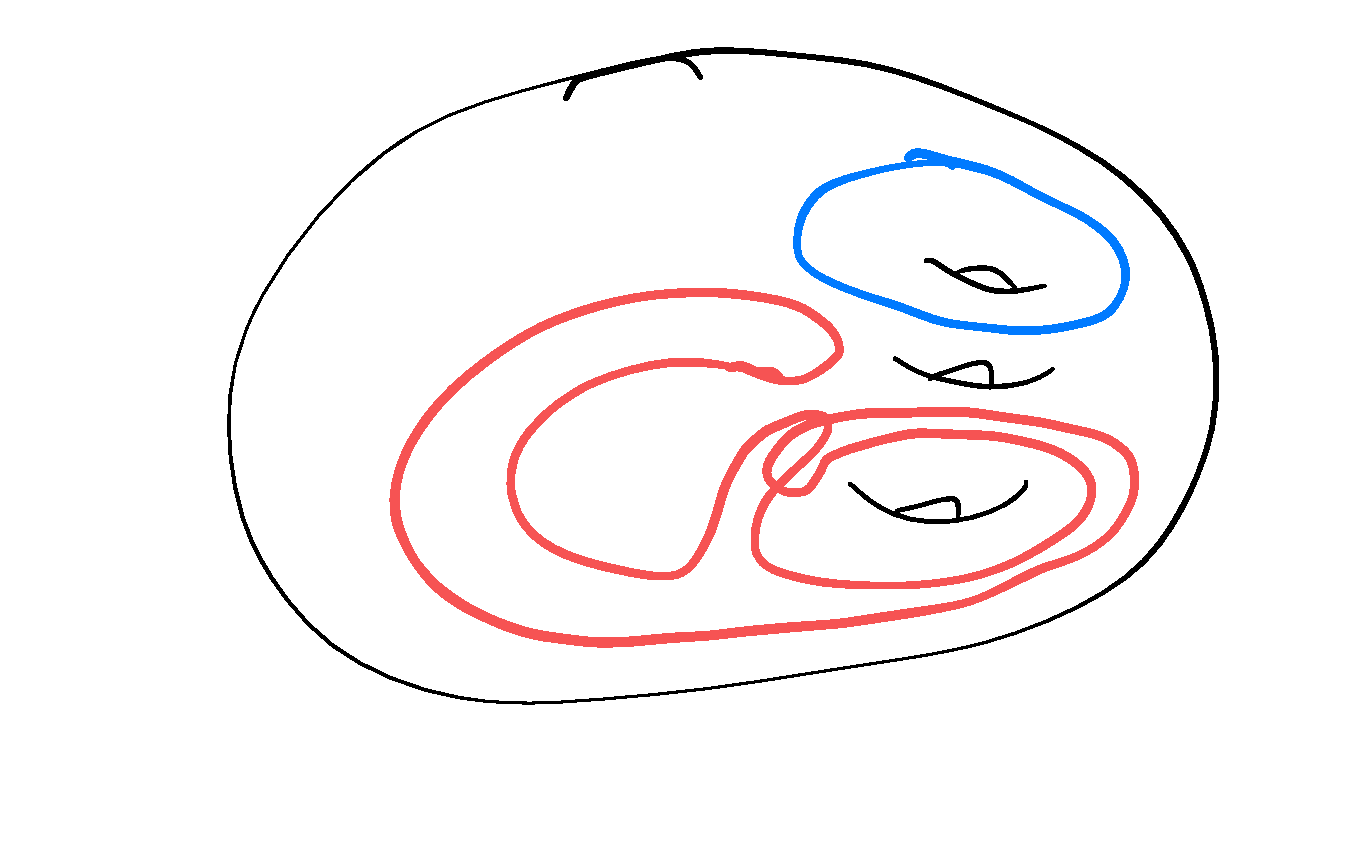
\includegraphics[width=.3\textwidth]{homotopy/contractable}
\caption{The blue curve is not contractable, the red curve is contractable.}
\label{fig:contractable}
\end{figure}

In this application, we will use a modified version
of the Gauss-Bonnet theorem. Given a combinatorial surface
$S$ define the curvature of a face to be $k(f)=1-\sum \beta_f$,
$k(v)=1-\frac{1}{2}\deg(v)+\sum_{v\in V} \alpha_v$.
Summing over all faces and vertices in $S$ gives,
\begin{theorem}[Modified Gauss-Bonnet]\label{thm:modify-g-b}
For a combinatorial surface $S$,
$\sum_{f\in F} k(f)+\sum_{v\in V}k(v)=\chi(S).$
\end{theorem}

\begin{proof}

$$\sum_{f\in F} k(f)+\sum_{v\in V}k(v)=|F|-\sum_{v\in V}\alpha_v + |V|-|E|+\sum_{v\in V}\alpha_v=\chi(S).$$
\end{proof}


Here, a we have a combinatorial surface that we call a map denoted $S$
with genus $g\geq 2.$ The case $g=0$ is the sphere where every curve
is contractible and when $g=1$ contractibility can be determined by a counting
argument\todo{explain}.
A curve is a closed walk, given as alternating sequence of vertices
and edges in $S$.
A \EMPH{homotopy} between two closed curves $\gamma_1$ and $\gamma_2$ that 
share a point $p_0$ is a continuous map $H\colon [0,1]\times \Sp^1 \to \mathbb{R}^2$ 
such that $H(0,\cdot)=\gamma_1$, $H(1,\cdot)=\gamma_2$, and $H(s,0)=p_0=H(s,1)$.

On a combinatorial surface, homotopies can be decomposed
into discrete moves called edge spikes, edge unspikes  and face flips.
The question we consider is: Given a closed walk $W$ in a map $\Sigma$ is there a finite
sequence of moves that reduces the curve to a trivial walk?


First, we transform $S$ into a simpler object called a system of loops.  
Let $T$ be a spanning tree of $S$, let $C$ be the edges in a co-tree
(a spanning tree of the dual), and let $L$ denote the left over edges,
Each edge in $S$ is in one of $(T,L,C)$.
Contract edges in $T$, delete edges in $C$ a system of loops $\Delta$.
When we contract and delete edges in $S$ we might affect edges in our walk $W$.
If we contract an edge in $W$, delete the edge from $W$.
If we delete and edge $e\in W$, face flip to avoid the deleted edge.
Get a new walk $W' \in \Delta$ homotopic to $W\in \Sigma$
now only haveing one vertex. Then, $W'$ has one vertex
with degree $4g$, one face with $4g$ edges, and $2g$ loops.
The length of the walk increases by at most $2g$.


The universal covering space of $S$ denoted $U$ is a plane
and when $g\geq 2$ $U$ has a natural hyperbolic geometry,
tiled by $4g$-gons.


Big idea: a curve is contractible closed walk in $S$
if and only if the walk is closed $U$.
Thus, our problem is equivalent to the following: Given a walk
in the universal cover of a system of loops, is it closed?

Here the walk is given as a starting vertex then we have a list of which
edges to take at each intermediate vertex. 
All vertices look the same, so we must determine if we have ended where
we began. 

Look for spurs or taking and instances where we talk the long way around a face, 
shorten the walk.
Any nontrivial contractible cycle contains either a spur or a bracket \cite{gertsen-short-1990}.
\begin{lemma}[Dehn's Lemma]\label{lem:dehn}
If $g\geq 2,$ then any nontirival closed walk has either a spur
or $4g-2$ consecutive edges on the boundary of a face.
\end{lemma}
\begin{proof}
Sketch: 
Any nontrival closed walk bounds a disk $D$ with $\chi(D)=1$, by the Gauss-Bonnet theorem
$$\sum_v k(v)+\sum_f k(f) =1.$$

Each face has $4g$ edges, each internal vertex has degree $4g$
and each  boundary vertex  has degree less than $4g$.
The angle of each angle on a face  is $\frac{1}{4}$,
thus, $k(f)=1-g<0,$ for internal vertices  $k(v)=1-g<0$ and for all
vertices on the boundary, $k(v)=\frac{3}{4}-\frac{\deg(v)}{4}$.
Boundary vertices fall into three  categories: convex, where $k(v)=\frac{1}{4}$
flats,  where $k(v)=0$  and concave where $k(v)<0$.

By G-B, $$|F|(1-g)+|v_{convex}|\frac{1}{4}\geq 1$$
and 
$$|v_{convex}|\geq (4g-4)|F|+4.$$

We divide by $|F|$ to determine the average number
of convex vertices per face to be greater than $4g-4$.
Thus, there exists some face that has $4g-3$ consecutive edges in the walk.
\end{proof}

This gives an algorithm for determining if a walk is closed in the universal
covering space.
Look for spurs and long boundary subpaths, the walk is closed if and  only if
we can  shrink the curve.
Label edges, walk is a sequence of labels
look at intervals of $4g-2$ in a walk, $8g$ paths
that represent long boundary paths, $4g$ spurs.
Slide window and look for spurs or long boundary paths.
If you find one remove it.

Brute force $O(g^3\ell)$ overall.
Can speed it up with Erickson DFA  idea
$O(g^2+g\ell)$.
Overall runtime $O(n+g^2+g\ell)$ time.

In trouble if $g$is big. Erickson uses system of quads,
radial map, $O(n)$ runtime  \cite{erickson-whittlesey-2013}.





